\documentclass{math}

\usepackage{tikz}
\usetikzlibrary{decorations.pathmorphing}

\title{University Physics 1A}
\author{Alvin Lin}
\date{December 4th, 2017}

\begin{document}

\maketitle

\section*{Pendulum Lab}
\begin{center}
  \begin{tikzpicture}
    \draw (3,0) -- node[pos=0.5, right] {\( L \)}
      (0,5.19) -- node[pos=0.5, left] {\( L \)}
      (-3,0) -- node[pos=0.5, below] {\( L \)} cycle;
    \draw[dashed] (0,0) -- (0,5.19);
    \draw[|<->|,thick] (-3.5,0) -- (-3.5,5.19) node[pos=0.5,left]
      {\( h = \frac{\sqrt{3}}{2}L \)};
    \node[fill,red,circle,inner sep=2pt,label={above:pivot}] at (0,5.19) {};
    \draw[dashed] (3,0) -- (4,0) node[right] {\( y = 0 \)};
    \node[fill,circle,inner sep=2pt] at (0,1.73) {};
    \draw[dashed] (0,1.73) -- (4,1.73)
      node[right] {\( y_{CoM} = \frac{1}{3}h = \frac{\sqrt{3}}{6}L\)};
  \end{tikzpicture}
\end{center}
\begin{align*}
  y_{CoM} &= \frac{1}{3}\frac{\sqrt{3}}{2}L \\
  &= \frac{\sqrt{3}}{6}L \\
  I_{CoM} &= 3\left[\frac{1}{12}mL^2+
    m\left(\frac{\sqrt{3}}{6}L\right)^2\right] \\
  &= \frac{1}{2}mL^2
\end{align*}
\begin{align*}
  I_{around~pivot} &= I_{CoM}+3(h-\frac{\sqrt{3}}{6})^2 \\
  &= \frac{1}{2}mL^2+3\left(\frac{\sqrt{3}}{3}L\right)^2 \\
  &= \frac{3}{2}mL^2 \\
  T &= \frac{2\pi}{\omega} \\
  &= \frac{2\pi}{\sqrt{\frac{y_{CoM}Mg}{I_{around~pivot}}}} \\
  &= 2\pi\sqrt{\frac{I_{around~pivot}}{y_{CoM}Mg}} \\
  &= 2\pi\sqrt{\frac{3}{2}mL^2\frac{6}{\sqrt{3}L}\frac{1}{(3m)g}} \\
  &= 2\pi\sqrt{\frac{\sqrt{3}}{2}\frac{L}{g}} \\
\end{align*}

\subsection*{Simple Harmonic Motion}
Generally, we think of masses oscillating on a spring in terms of simple
harmonic motion. This can be described with the following equation of motion:
\begin{align*}
  F &= -kx \\
  a &= -\frac{k}{m}x \\
  x &= A\cos(\omega t+\phi) \\
  v &= -\omega A\sin(\omega t+\phi) \\
  \omega &= \sqrt{\frac{k}{m}}
\end{align*}
Total Mechanical Energy:
\begin{align*}
  KE+PE &= \frac{1}{2}mv^2+\frac{1}{2}kx^2 \\
  &= \frac{1}{2}m\omega^2A^2\sin^2(\omega t+\phi)+
    \frac{1}{2}kA^2\cos^2(\omega t+\phi) \\
  &= \frac{1}{2}m(\frac{k}{m})A^2\sin^2(\omega t+\phi)+
    \frac{1}{2}kA^2\cos^2(\omega t+\phi) \\
  &= \frac{1}{2}kA^2\bigg(\sin^2(\omega t+\phi)+\cos^2(\omega t+\phi)\bigg) \\
  &= \frac{1}{2}kA^2
\end{align*}
Because of the properties of the sinusoidal curves, the maximum kinetic energy
occurs at \( \omega t+\phi = \frac{\pi}{2},\frac{3\pi}{2},\frac{5\pi}{2},\dots
\) and the maximum potential energy at \( \omega t+\phi = 0,\pi,2\pi,\dots \).

\subsection*{Waves}
Mechanical waves occur in the form of oscillating springs, strings, and ropes.
In nature we can observe seismic waves, water waves, and sound waves. Waves also
occur as electromagnetic waves where energy and magnetism oscillate. They occur
as transverse or longitudinal waves.
\begin{center}
  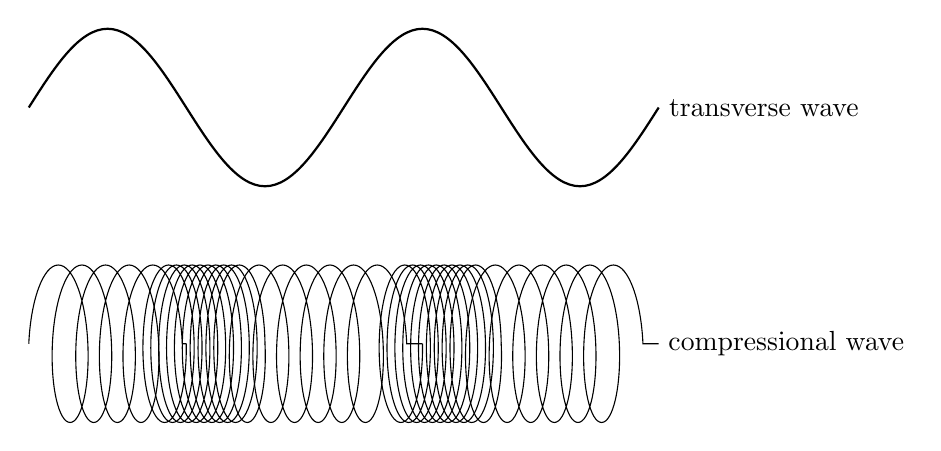
\begin{tikzpicture}[decoration={coil}]
    \draw[thick] (0,0) sin (1,1) cos (2,0) sin (3,-1) cos (4,0) sin (5,1) cos
      (6,0) sin (7,-1) cos (8,0) node[right] {transverse wave};
    \draw[decorate, decoration={aspect=0.3, segment length=3mm, amplitude=1cm}] (0,-3) --(2,-3);
    \draw[decorate, decoration={aspect=0.3, segment length=1mm, amplitude=-1cm}]
      (2,-3) -- (3,-3);
    \draw[decorate, decoration={aspect=0.3, segment length=3mm, amplitude=-1cm}]
      (3,-3) -- (5,-3);
    \draw[decorate, decoration={aspect=0.3, segment length=1mm, amplitude=-1cm}]
      (5,-3) -- (6,-3);
    \draw[decorate, decoration={aspect=0.3, segment length=3mm, amplitude=-1cm}]
      (6,-3) -- (8,-3) node[right] {compressional wave};
  \end{tikzpicture}
\end{center}
Waves are represented using the following equation:
\[ y = y_{max}\cos(kx-\omega t) \]
where \( y_{max} \) is the amplitude, \( k \) is the angular wave number in
radians per meter, and \( \omega \) is the angular frequency in radians per
second. The distance between one part of the wave to the next identical part
in the wave is the wavelength, represented by \( \lambda \). The time between
those occurrences at one position is the period \( T \).
\begin{center}
  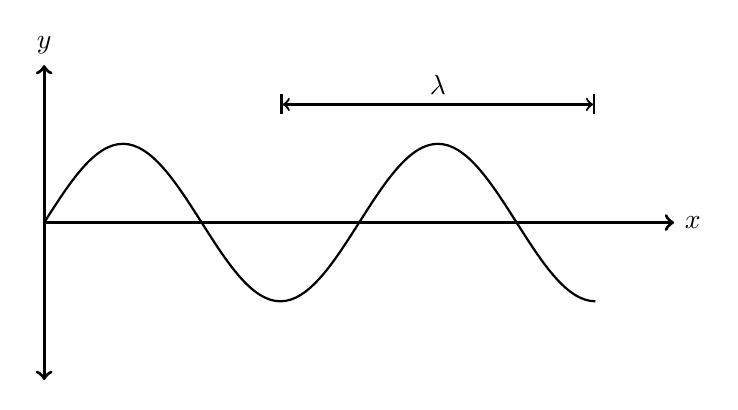
\begin{tikzpicture}
    \draw[<->,very thick] (0,-2) -- (0,2) node[above] {\( y \)};
    \draw[->,very thick] (0,0) -- (8,0) node[right] {\( x \)};
    \draw[thick] (0,0) sin (1,1) cos (2,0) sin (3,-1) cos (4,0) sin (5,1) cos (6,0) sin (7,-1);
    \draw[|<->|,thick] (3,1.5) -- (7,1.5) node[pos=0.5,above] {\( \lambda \)};
  \end{tikzpicture}
    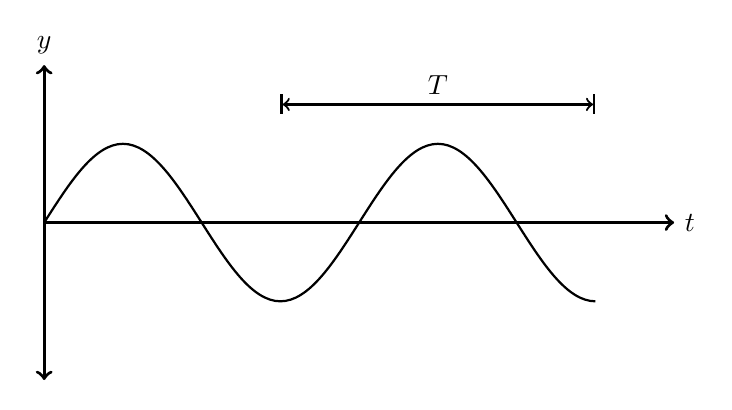
\begin{tikzpicture}
      \draw[<->,very thick] (0,-2) -- (0,2) node[above] {\( y \)};
      \draw[->,very thick] (0,0) -- (8,0) node[right] {\( t \)};
      \draw[thick] (0,0) sin (1,1) cos (2,0) sin (3,-1) cos (4,0) sin (5,1) cos (6,0) sin (7,-1);
      \draw[|<->|,thick] (3,1.5) -- (7,1.5) node[pos=0.5,above] {\( T \)};
    \end{tikzpicture}
\end{center}
\begin{align*}
  2\pi &= k\lambda \\
  k &= \frac{2\pi}{\lambda} \\
  2\pi &= \omega T \\
  T &= \frac{2\pi}{\omega} = \frac{1}{f}
\end{align*}
We can derive the position function to determine the velocity of a particle in
the wave.
\begin{align*}
  y &= y_{max}\cos(kx-\omega t) \\
  v &= \ddiff{y}{t} \\
  &= \omega y_{max}\sin(kx-\omega t)
\end{align*}

\subsection*{Wave Pattern}
The wave is a pattern that moves.
\begin{center}
  \begin{tikzpicture}
    \draw[->,very thick] (0,0) -- (0,-5) node[below] {\( t \)};
    \draw[->,very thick] (0,0) -- (5,0) node[right] {\( x \)};
    \draw (1,-2) -- (2,-2) sin (2.5,-1.5) cos (3,-2) -- (5,-2);
    \draw (1,-4) -- (3,-4) sin (3.5,-3.5) cos (4,-4) -- (5,-4);
  \end{tikzpicture}
\end{center}
\begin{align*}
  y &= y_{max}\cos(kx-\omega t) \\
  \ddiff{}{t}(kx-\omega t) &= 0 \\
  k\ddiff{x}{t}-\omega &= 0 \\
  \ddiff{x}{t} &= \frac{\omega}{k}
\end{align*}
The points in the wave stay constant as the wave moves. This derivative in terms
of time is the speed of the wave pattern. \( y = y_{max}\cos(kx-\omega t) \)
represents the wave moving in the positive direction and \( y =
y_{max}\cos(kx+\omega t) \) represents the wave moving in the negative
direction.

\begin{center}
  You can find all my notes at \url{http://omgimanerd.tech/notes}. If you have
  any questions, comments, or concerns, please contact me at
  alvin@omgimanerd.tech
\end{center}

\end{document}
